\documentclass{article}
\usepackage[utf8]{inputenc}

\title{MP5 Report}
\author{Rafal Stapinski}
\date{December 12 2018}
\usepackage{graphicx}
\begin{document}

\maketitle

\section{a.1}

Time update step \newline \newline

$\hat{x}^{-}_{k} = A \hat{x}_{k-1} + B u_{k-1} $ where A, B are 2x2 identity matrices, and $u_{k-1}$ is the vector $[u_{1,k-1}, u_{2,k-1}]$ \newline \newline

$P^{-}_{k} = A P_{k-1}A^{T} + Q$ where Q is the given system noise \newline \newline
Measurement update step \newline \newline

$\hat{x}_k = \hat{x}^{-}_{k} + K_k(z_k - H\hat{x}^-_k)$ where H is a 2x2 identity matrix, $z_k$ is the vector $[z_{1,k}, z_{2,k}]$ \newline \newline

$K_k = \frac{P^{-}_{k}H^T}{HP^-_k H^T + R}$ where R is the given measurement noise \newline \newline

$P_k = (I - K_k H)P^-_k$ \newline \newline

\newpage
\section{a.4}
The value of $\lambda$ that seemed to consistently give the best results was small, and ultimately 0.1 \newline

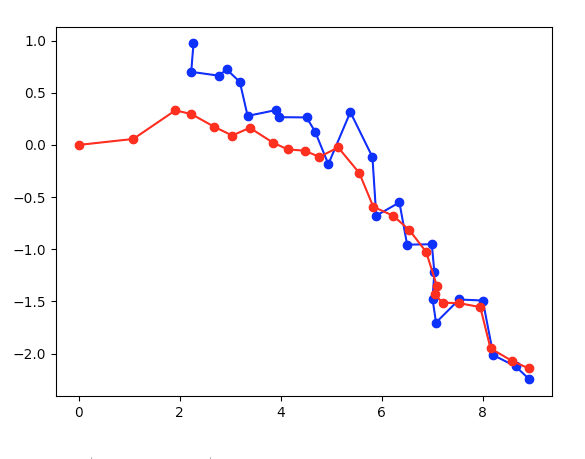
\includegraphics[scale=0.4]{plot.png}

\section{b.2}
kalman2d\_shoot uses the kalman2d function. It uses the R and Q used by the game. It decides when to shoot by looking at recent observed and predicted pairs. If recent estimates have accurately predicted future observed values, the function decides that now is a good time to shoot.

\end{document}
